\item \textbf{Separate the  various  activities  and  visualize  the  data  for  the  different  classes.  Next,  explore  using HMM  state  modeling  for  each activity (‘Standing  Up,  Walking  and  Going  up-down  stairs’)  by breaking  the activity into different states (for example 3 states, one for ‘Standing Up’  ,  a second for ‘Walking’  and a third  for  ‘Going  up-down  stairs’).  Analyze  the  results  of fitting  the  model  for different  HMM  states  by visual  inspection  (since  no  ground  truths  are available for where  a  sub-activity  starts  and  ends).  Generate  these  qualitative  results  for  state  decoding  when training  on  users 1-10, and testing  on users 11-15.}
The dataset collected data from an accelerate sensor carried by different users. Data were separated by participant in different CSV files. Each row in these files contains the information of sequential number (time), x, y, z acceleration, and label. Label took a number between 1 and 7 according to the user activity. Table \ref{tab:activity} shows these activities along with the codes.
\begin{table}[H]
\centering
\caption{The dataset activity and label code.}
\label{tab:activity}
\begin{tabular}{rl}
\toprule
   Label value &  Activity \\
\midrule
  1 & Working at Computer               \\
  2 & Standing Up, Walking and Going Up-Down Stairs               \\
  3 & Standing                 \\
  4 & Walking     \\
  5 & Going Up-Down Stairs                \\
  6 & Walking and Talking with Someone                    \\
  7 & Talking while Standing          \\

\bottomrule
\end{tabular}

\end{table}
For the rest of this assignment, we used a Pandas DataFrame for separating and storing the data and named it DF1. Figure \ref{fig:Ass3_Q2_raw_signal_2} shows signals of x, y, z, and label for the last participant.
\begin{figure}[H]
    \centering
    \begin{minipage}[b]{1\textwidth}
        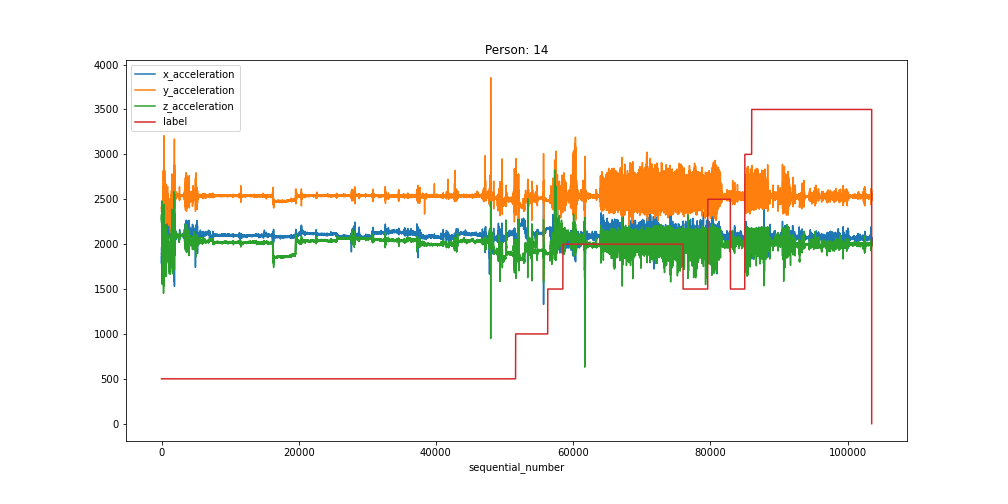
\includegraphics[width=\textwidth]{figures/Ass3/Ass3_Q2_raw_signal_21.png}
    \end{minipage}
    \caption{The signals of x, y, z, and label for the last participant. For better understanding, the code of each activity multiply by 500.}
    \label{fig:Ass3_Q2_raw_signal_2}
\end{figure}

Figures \ref{fig:Ass3_Q3_raw_signal} and \ref{fig:Ass3_Q2_raw_signal} show the raw signal that were filtered based on different users and activities.

\begin{figure}[H]
    \centering
    \begin{minipage}[b]{1\textwidth}
        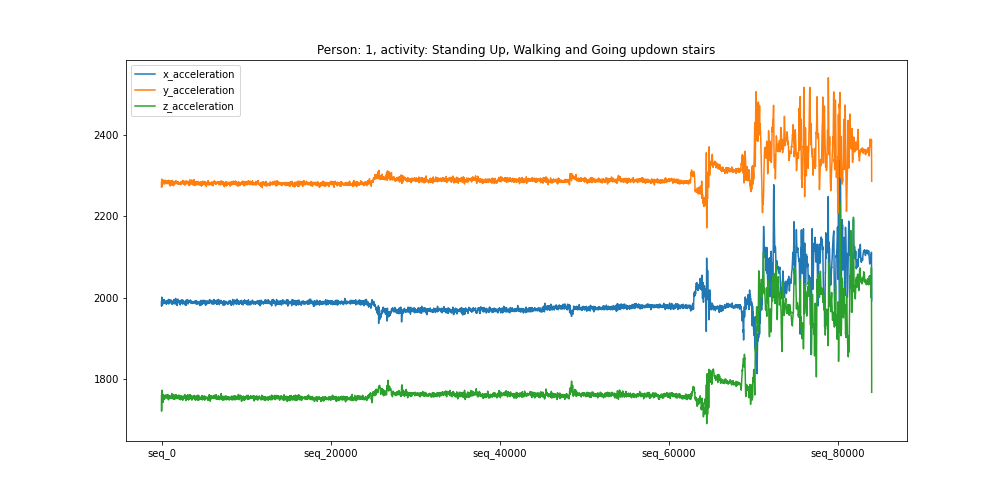
\includegraphics[width=\textwidth]{manuscript/src/figures/Ass3/Ass3_Q3_raw_signal.png}
    \end{minipage}
    \caption{The signals of x, y, and z for the first participant and ‘Standing  Up,  Walking  and  Going  up-down  stairs’ activity.}
    \label{fig:Ass3_Q3_raw_signal}
\end{figure}
\begin{figure}[H]
    \centering
    \begin{minipage}[b]{1\textwidth}
        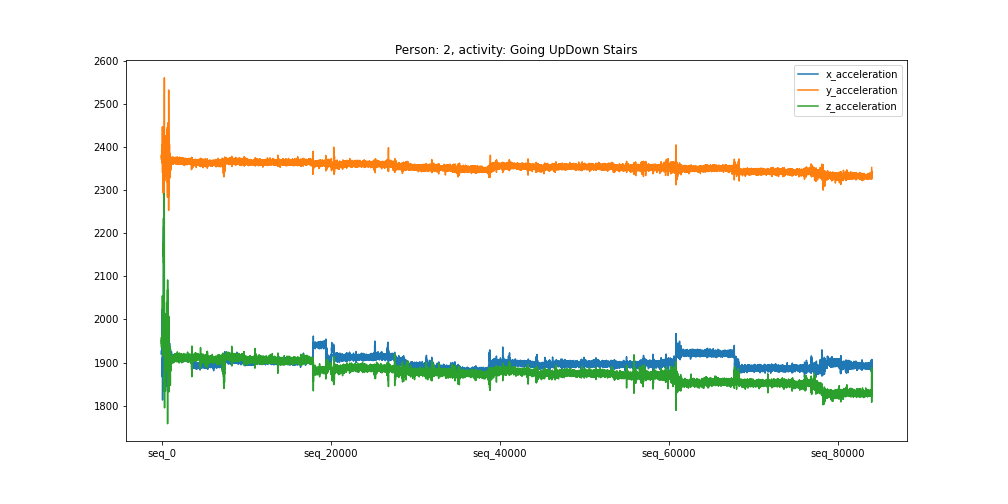
\includegraphics[width=\textwidth]{manuscript/src/figures/Ass3/Ass3_Q2_raw_signal.png}
    \end{minipage}
    \caption{The signals of x, y, and z for the second participant and ‘Going  up-down  stairs’ activity.}
    \label{fig:Ass3_Q2_raw_signal}
\end{figure}

The next part of this question is a decoding problem. We had an activity that was included different states (walking, standing, and going up-down stairs). Our goal is that to find the hidden states for this activity based on the observation signals.
Before going into model detail, let first talk about the pre processing step. In this step, first we separated and resized all signals of ‘Standing  Up,  Walking  and  Going  up-down  stairs’ from the dataset. Then, this data were stored in an array with shape of $15 \times 840000 \times 3$. The dimensions of this array show the number of users,  samples, and observation signals respectively.
For training part, we separated the array by different users. the first ten users were used as training set and others considered for testing the model. Figures \ref{Ass3_Q2_states_user_0} to \ref{fig:Ass3_Q2_states_user_14} demonstrate the results of HMM on all users data. Besides, to find the effect of data scale, we used normalized data ( see figures \ref{fig:Ass3_Q2_states_user_0N} to \ref{fig:Ass3_Q2_states_user_14N}).
\begin{figure}[H]
    \centering
    \begin{minipage}[b]{1\textwidth}
        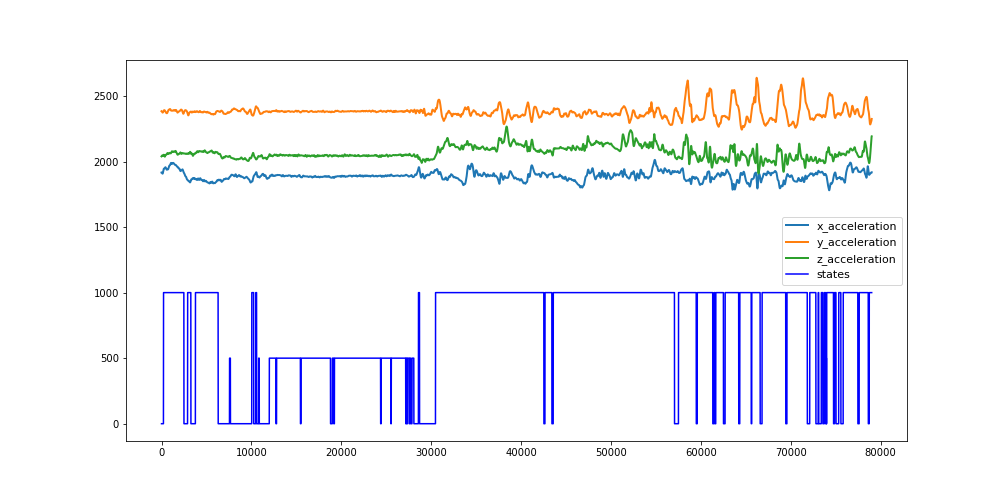
\includegraphics[width=\textwidth]{manuscript/src/figures/Ass3/Ass3_Q2_states_user_0.png}
    \end{minipage}
    \caption{The signals of x, y, and z for participant 1 and ‘Standing  Up,  Walking  and  Going  up-down  stairs’ activity. The dark blue signal indicates the different states.}
    \label{fig:Ass3_Q2_states_user_0}
\end{figure}
\begin{figure}[H]
    \centering
    \begin{minipage}[b]{1\textwidth}
        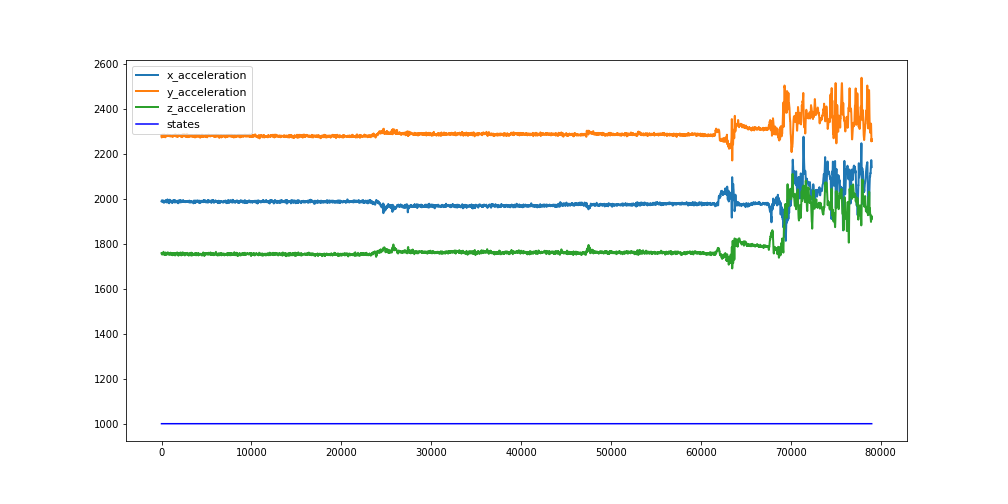
\includegraphics[width=\textwidth]{manuscript/src/figures/Ass3/Ass3_Q2_states_user_1.png}
    \end{minipage}
    \caption{The signals of x, y, and z for participant 2 and ‘Standing  Up,  Walking  and  Going  up-down  stairs’ activity. The dark blue signal indicates the different states.}
    \label{fig:Ass3_Q2_states_user_1}
\end{figure}
\begin{figure}[H]
    \centering
    \begin{minipage}[b]{1\textwidth}
        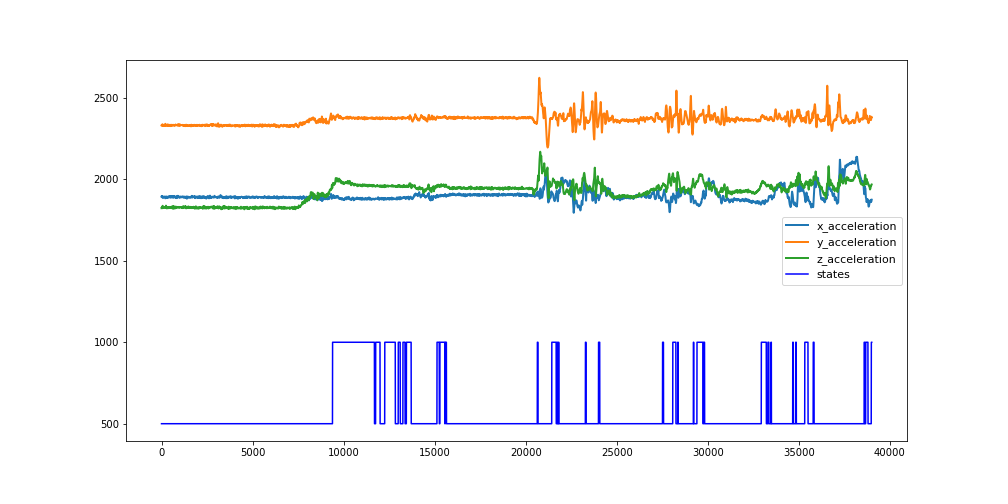
\includegraphics[width=\textwidth]{manuscript/src/figures/Ass3/Ass3_Q2_states_user_2.png}
    \end{minipage}
    \caption{The signals of x, y, and z for participant 3 and ‘Standing  Up,  Walking  and  Going  up-down  stairs’ activity. The dark blue signal indicates the different states.}
    \label{fig:Ass3_Q2_states_user_2}
\end{figure}
\begin{figure}[H]
    \centering
    \begin{minipage}[b]{1\textwidth}
        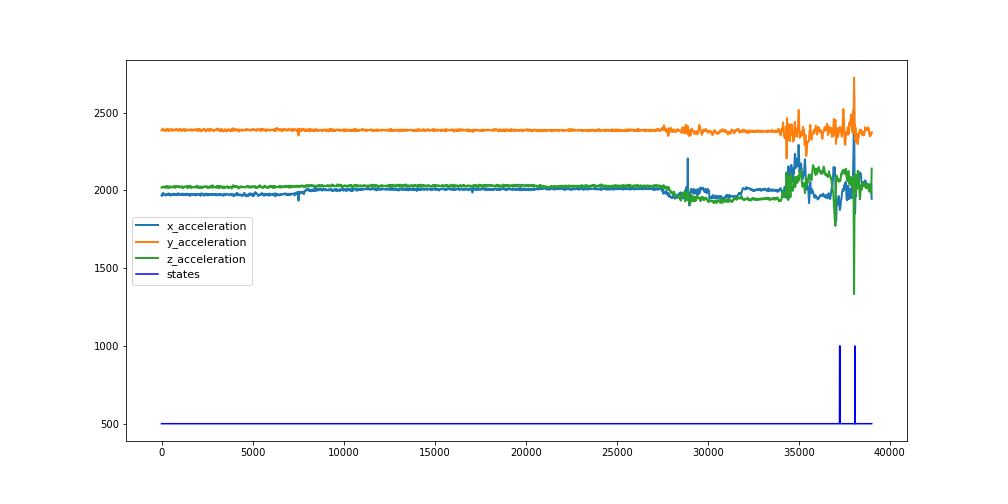
\includegraphics[width=\textwidth]{manuscript/src/figures/Ass3/Ass3_Q2_states_user_3.png}
    \end{minipage}
    \caption{The signals of x, y, and z for participant 4 and ‘Standing  Up,  Walking  and  Going  up-down  stairs’ activity. The dark blue signal indicates the different states.}
    \label{fig:Ass3_Q2_states_user_3}
\end{figure}
\begin{figure}[H]
    \centering
    \begin{minipage}[b]{1\textwidth}
        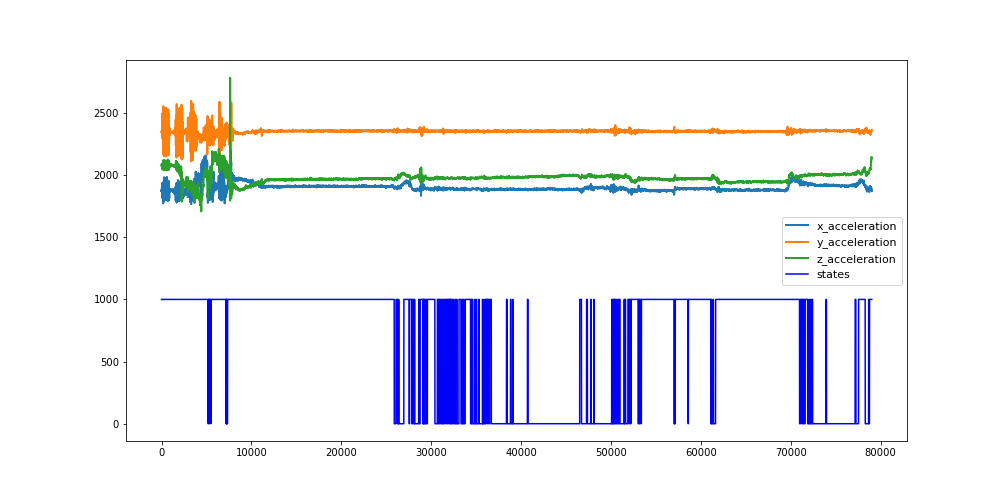
\includegraphics[width=\textwidth]{manuscript/src/figures/Ass3/Ass3_Q2_states_user_4.png}
    \end{minipage}
    \caption{The signals of x, y, and z for participant 5 and ‘Standing  Up,  Walking  and  Going  up-down  stairs’ activity. The dark blue signal indicates the different states.}
    \label{fig:Ass3_Q2_states_user_4}
\end{figure}
\begin{figure}[H]
    \centering
    \begin{minipage}[b]{1\textwidth}
        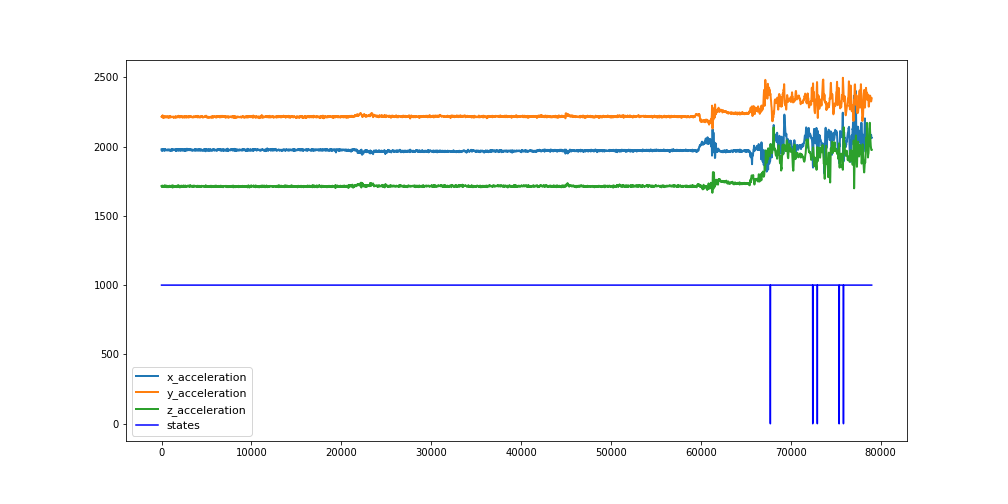
\includegraphics[width=\textwidth]{manuscript/src/figures/Ass3/Ass3_Q2_states_user_5.png}
    \end{minipage}
    \caption{The signals of x, y, and z for participant 6 and ‘Standing  Up,  Walking  and  Going  up-down  stairs’ activity. The dark blue signal indicates the different states.}
    \label{fig:Ass3_Q2_states_user_5}
\end{figure}
\begin{figure}[H]
    \centering
    \begin{minipage}[b]{1\textwidth}
        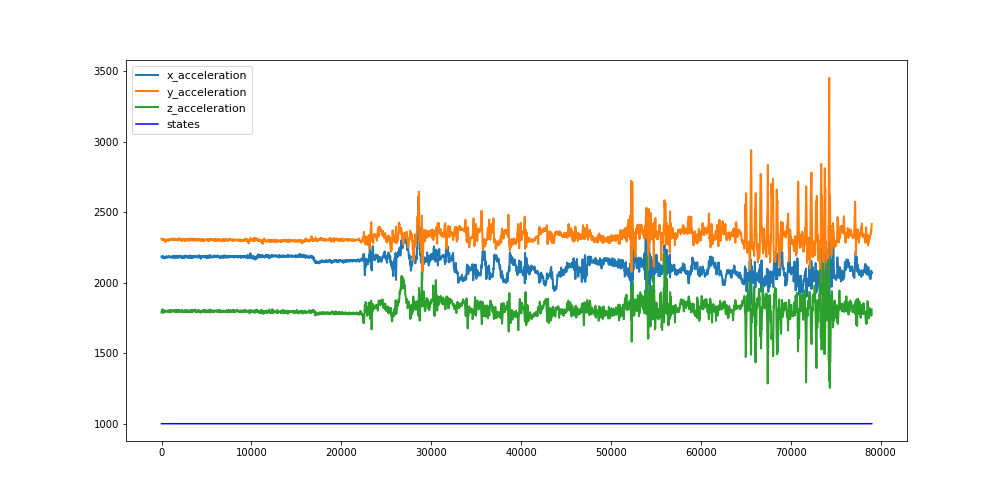
\includegraphics[width=\textwidth]{manuscript/src/figures/Ass3/Ass3_Q2_states_user_6.png}
    \end{minipage}
    \caption{The signals of x, y, and z for participant 7 and ‘Standing  Up,  Walking  and  Going  up-down  stairs’ activity. The dark blue signal indicates the different states.}
    \label{fig:Ass3_Q2_states_user_6}
\end{figure}
\begin{figure}[H]
    \centering
    \begin{minipage}[b]{1\textwidth}
        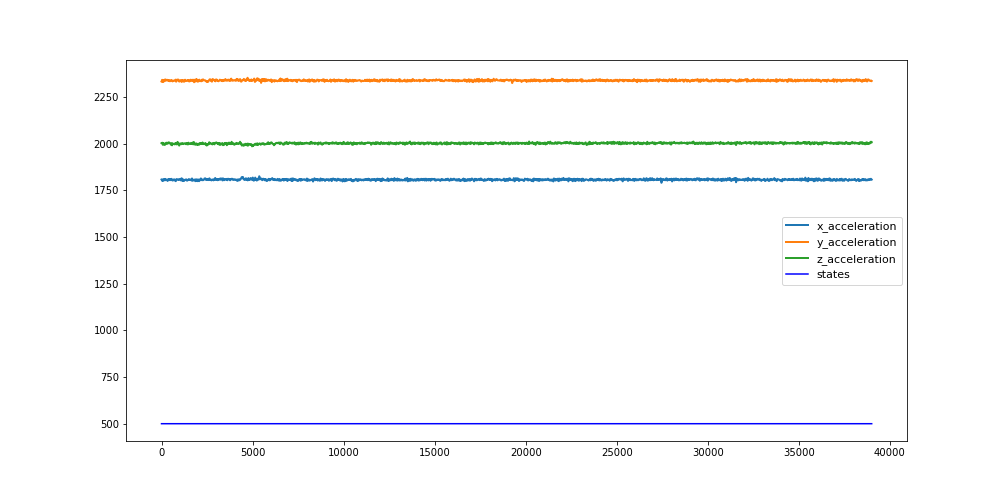
\includegraphics[width=\textwidth]{manuscript/src/figures/Ass3/Ass3_Q2_states_user_7.png}
    \end{minipage}
    \caption{The signals of x, y, and z for participant 8 and ‘Standing  Up,  Walking  and  Going  up-down  stairs’ activity. The dark blue signal indicates the different states.}
    \label{fig:Ass3_Q2_states_user_7}
\end{figure}
\begin{figure}[H]
    \centering
    \begin{minipage}[b]{1\textwidth}
        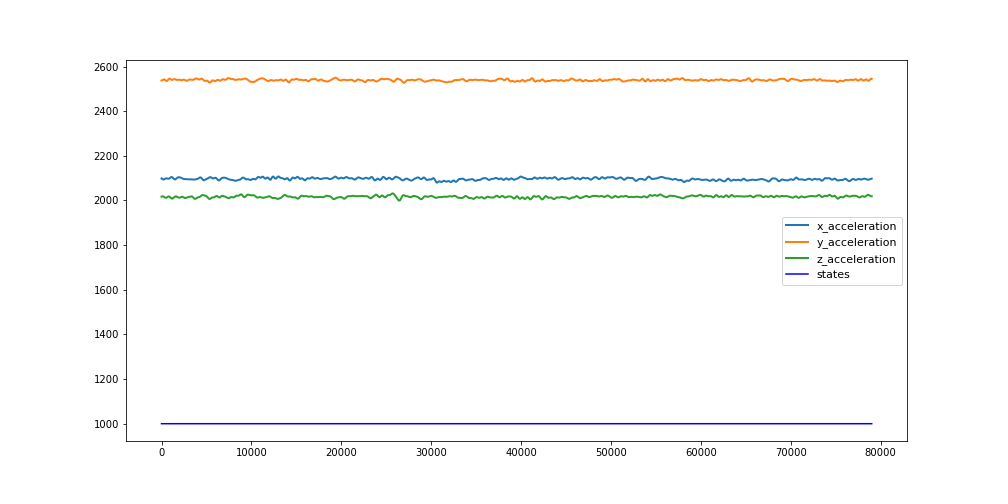
\includegraphics[width=\textwidth]{manuscript/src/figures/Ass3/Ass3_Q2_states_user_8.png}
    \end{minipage}
    \caption{The signals of x, y, and z for participant 9 and ‘Standing  Up,  Walking  and  Going  up-down  stairs’ activity. The dark blue signal indicates the different states.}
    \label{fig:Ass3_Q2_states_user_8}
\end{figure}
\begin{figure}[H]
    \centering
    \begin{minipage}[b]{1\textwidth}
        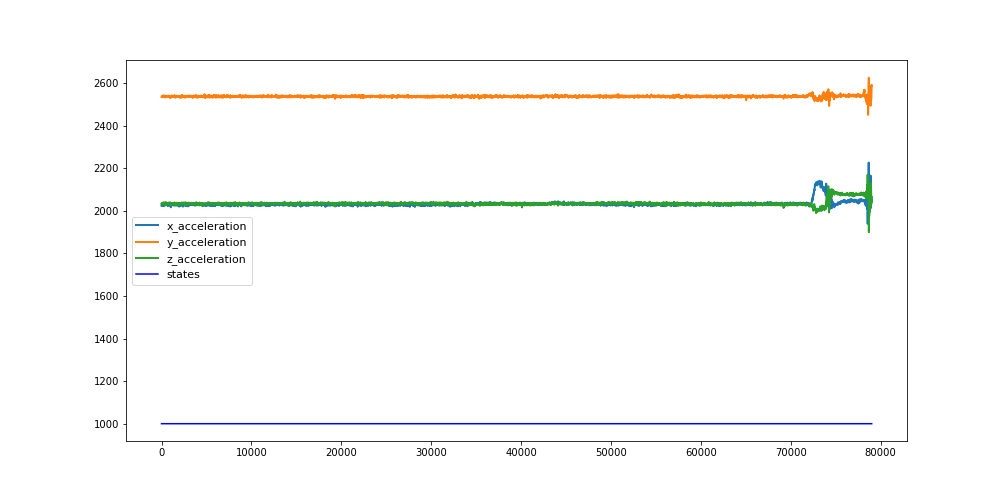
\includegraphics[width=\textwidth]{manuscript/src/figures/Ass3/Ass3_Q2_states_user_9.png}
    \end{minipage}
    \caption{The signals of x, y, and z for participant 10 and ‘Standing  Up,  Walking  and  Going  up-down  stairs’ activity. The dark blue signal indicates the different states.}
    \label{fig:Ass3_Q2_states_user_9}
\end{figure}
\begin{figure}[H]
    \centering
    \begin{minipage}[b]{1\textwidth}
        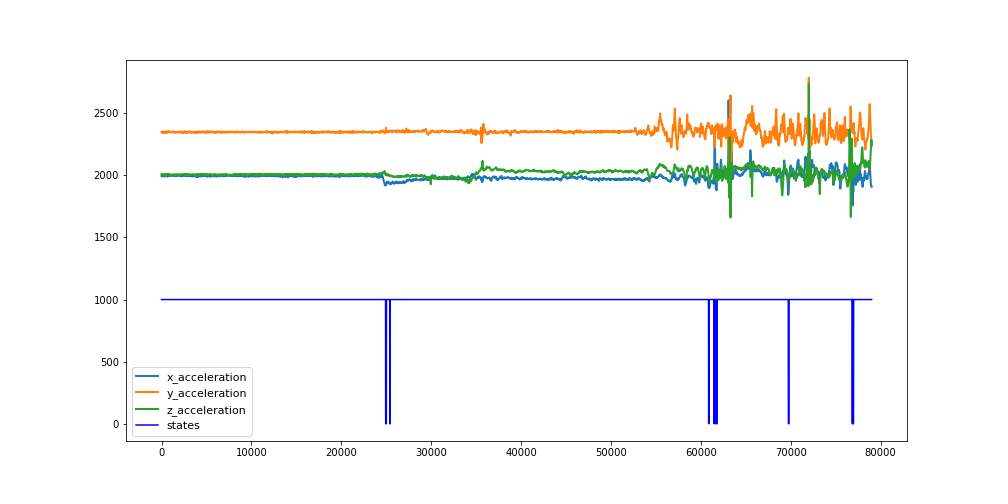
\includegraphics[width=\textwidth]{manuscript/src/figures/Ass3/Ass3_Q2_states_user_10.png}
    \end{minipage}
    \caption{The signals of x, y, and z for participant 11 and ‘Standing  Up,  Walking  and  Going  up-down  stairs’ activity. The dark blue signal indicates the different states.}
    \label{fig:Ass3_Q2_states_user_10}
\end{figure}
\begin{figure}[H]
    \centering
    \begin{minipage}[b]{1\textwidth}
        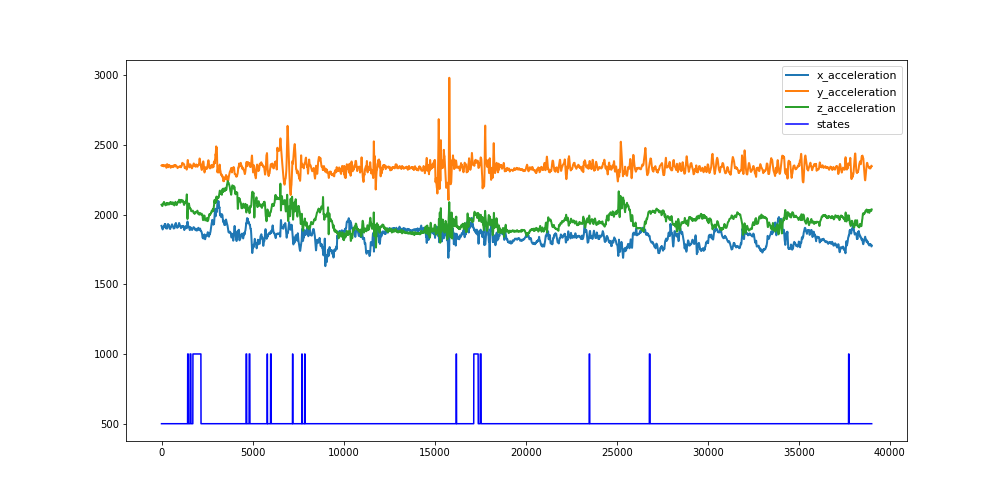
\includegraphics[width=\textwidth]{manuscript/src/figures/Ass3/Ass3_Q2_states_user_11.png}
    \end{minipage}
    \caption{The signals of x, y, and z for participant 12 and ‘Standing  Up,  Walking  and  Going  up-down  stairs’ activity. The dark blue signal indicates the different states.}
    \label{fig:Ass3_Q2_states_user_11}
\end{figure}
\begin{figure}[H]
    \centering
    \begin{minipage}[b]{1\textwidth}
        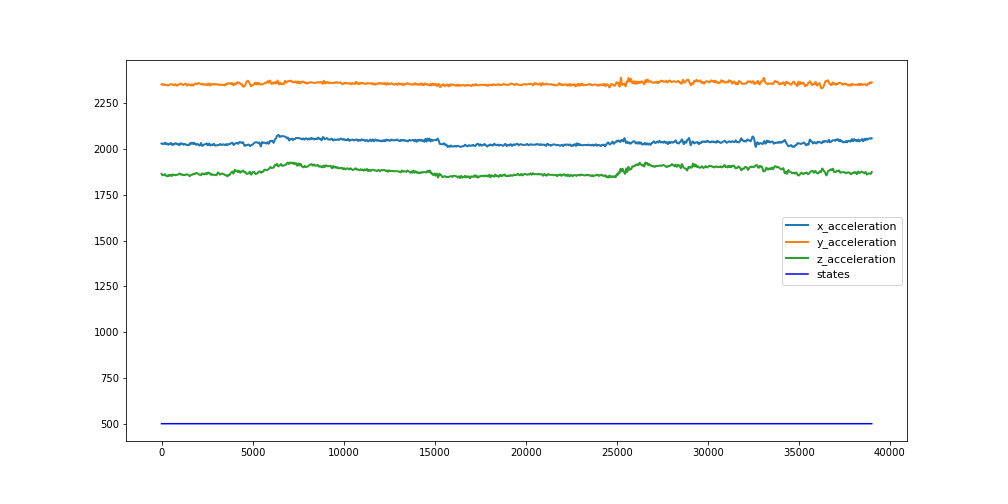
\includegraphics[width=\textwidth]{manuscript/src/figures/Ass3/Ass3_Q2_states_user_12.png}
    \end{minipage}
    \caption{The signals of x, y, and z for participant 13 and ‘Standing  Up,  Walking  and  Going  up-down  stairs’ activity. The dark blue signal indicates the different states.}
    \label{fig:Ass3_Q2_states_user_12}
\end{figure}
\begin{figure}[H]
    \centering
    \begin{minipage}[b]{1\textwidth}
        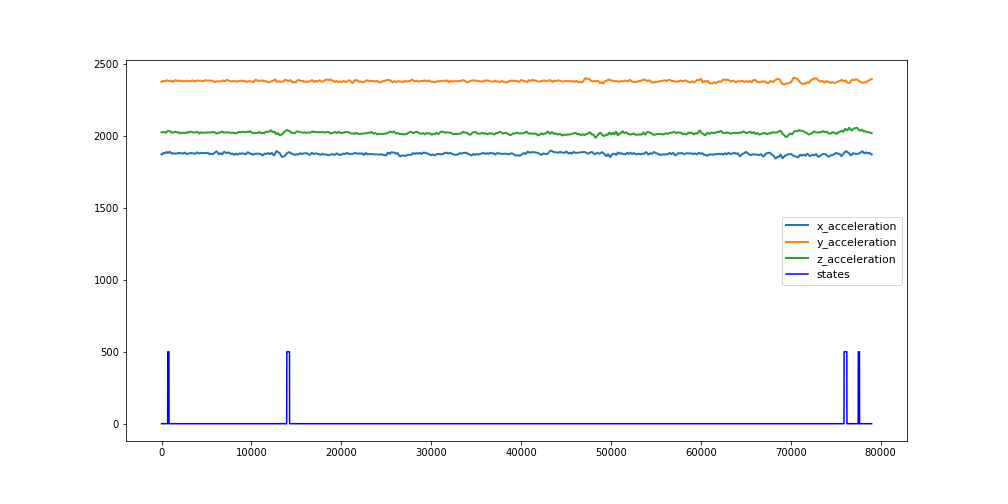
\includegraphics[width=\textwidth]{manuscript/src/figures/Ass3/Ass3_Q2_states_user_13.png}
    \end{minipage}
    \caption{The signals of x, y, and z for participant 14 and ‘Standing  Up,  Walking  and  Going  up-down  stairs’ activity. The dark blue signal indicates the different states.}
    \label{fig:Ass3_Q2_states_user_13}
\end{figure}
\begin{figure}[H]
    \centering
    \begin{minipage}[b]{1\textwidth}
        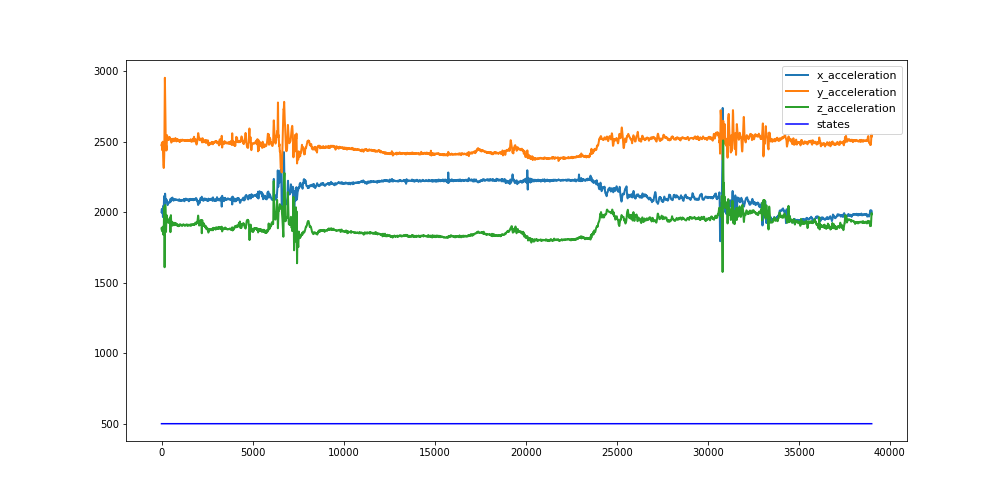
\includegraphics[width=\textwidth]{manuscript/src/figures/Ass3/Ass3_Q2_states_user_14.png}
    \end{minipage}
    \caption{The signals of x, y, and z for participant 15 and ‘Standing  Up,  Walking  and  Going  up-down  stairs’ activity. The dark blue signal indicates the different states.}
    \label{fig:Ass3_Q2_states_user_14}
\end{figure}
%%%%%%%%%%%%%%%%%%%%%%%%%%%%%%%%%%%%%%%%%%%%%%%%%%%%%%%%%%
\begin{figure}[H]
    \centering
    \begin{minipage}[b]{1\textwidth}
        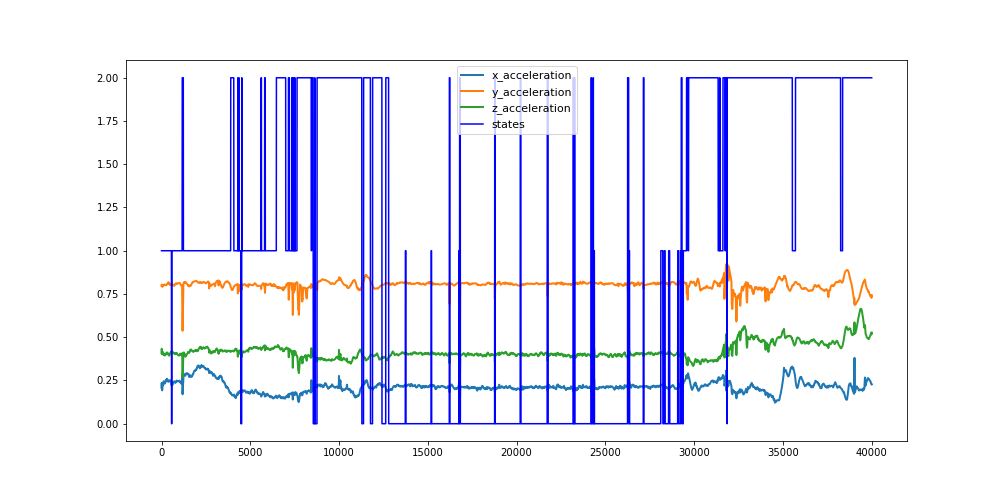
\includegraphics[width=\textwidth]{manuscript/src/figures/Ass3/Ass3_Q2_states_user_0N.png}
    \end{minipage}
    \caption{The normalized signals of x, y, and z for participant 1 and ‘Standing  Up,  Walking  and  Going  up-down  stairs’ activity. The dark blue signal indicates the different states.}
    \label{fig:Ass3_Q2_states_user_0N}
\end{figure}
\begin{figure}[H]
    \centering
    \begin{minipage}[b]{1\textwidth}
        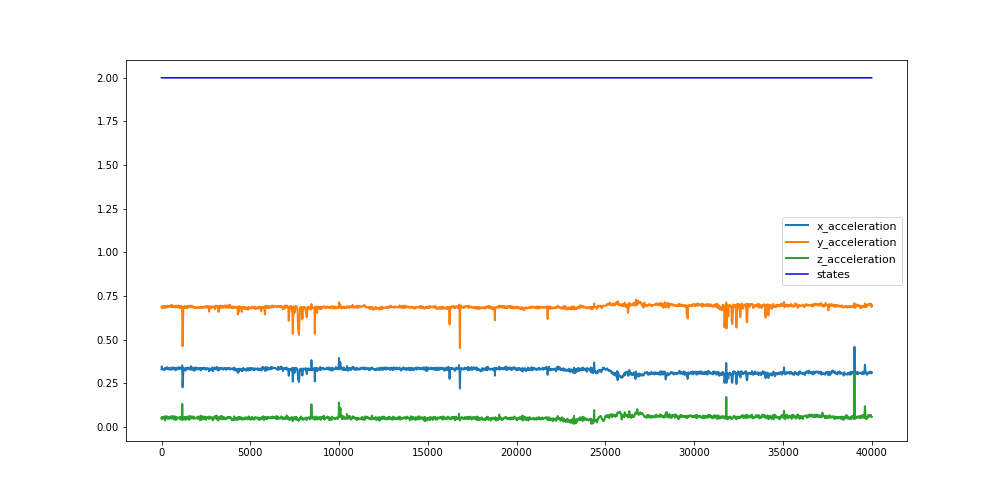
\includegraphics[width=\textwidth]{manuscript/src/figures/Ass3/Ass3_Q2_states_user_1N.png}
    \end{minipage}
    \caption{The normalized signals of x, y, and z for participant 2 and ‘Standing  Up,  Walking  and  Going  up-down  stairs’ activity. The dark blue signal indicates the different states.}
    \label{fig:Ass3_Q2_states_user_1N}
\end{figure}
\begin{figure}[H]
    \centering
    \begin{minipage}[b]{1\textwidth}
        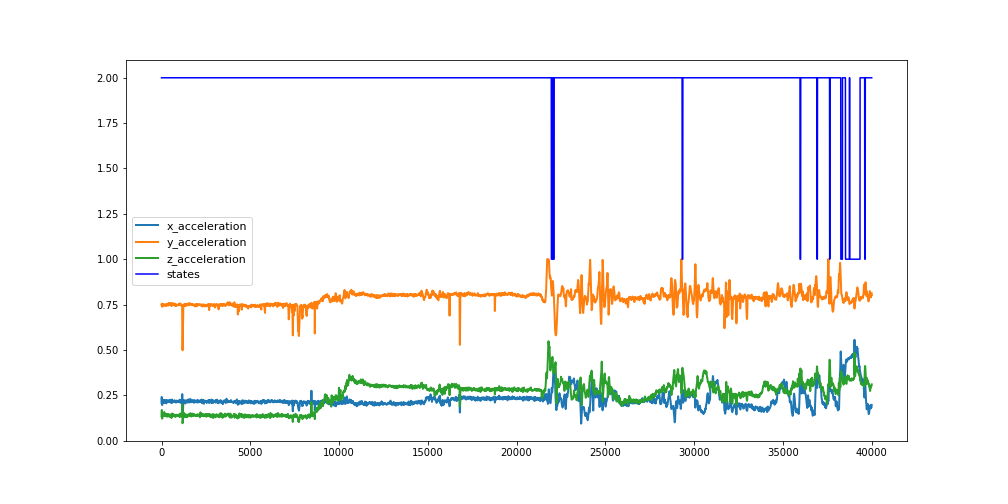
\includegraphics[width=\textwidth]{manuscript/src/figures/Ass3/Ass3_Q2_states_user_2N.png}
    \end{minipage}
    \caption{The normalized signals of x, y, and z for participant 3 and ‘Standing  Up,  Walking  and  Going  up-down  stairs’ activity. The dark blue signal indicates the different states.}
    \label{fig:Ass3_Q2_states_user_2N}
\end{figure}
\begin{figure}[H]
    \centering
    \begin{minipage}[b]{1\textwidth}
        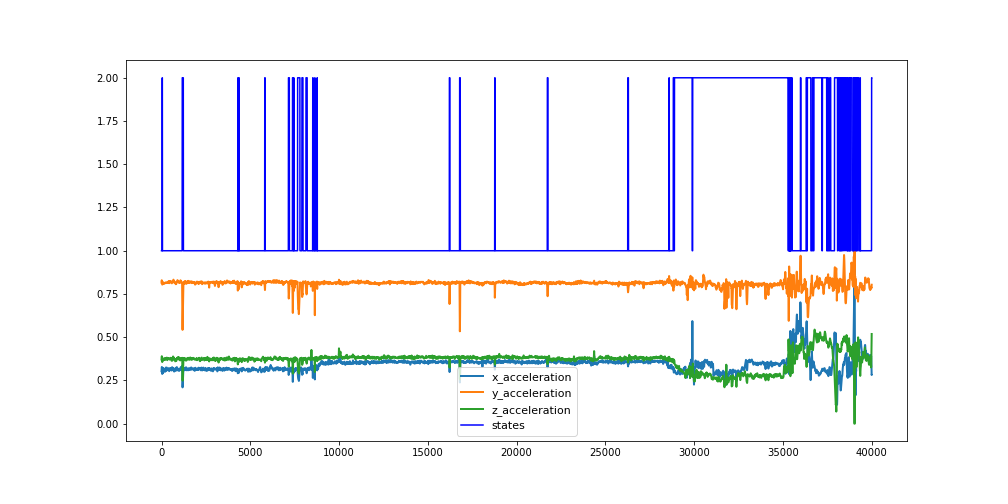
\includegraphics[width=\textwidth]{manuscript/src/figures/Ass3/Ass3_Q2_states_user_3N.png}
    \end{minipage}
    \caption{The normalized signals of x, y, and z for participant 4 and ‘Standing  Up,  Walking  and  Going  up-down  stairs’ activity. The dark blue signal indicates the different states.}
    \label{fig:Ass3_Q2_states_user_3N}
\end{figure}
\begin{figure}[H]
    \centering
    \begin{minipage}[b]{1\textwidth}
        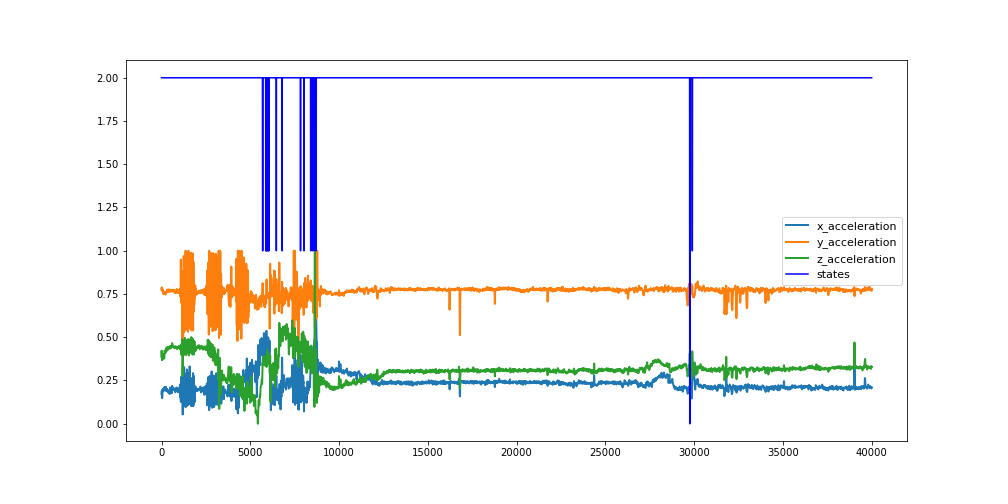
\includegraphics[width=\textwidth]{manuscript/src/figures/Ass3/Ass3_Q2_states_user_4N.png}
    \end{minipage}
    \caption{The normalized signals of x, y, and z for participant 5 and ‘Standing  Up,  Walking  and  Going  up-down  stairs’ activity. The dark blue signal indicates the different states.}
    \label{fig:Ass3_Q2_states_user_4N}
\end{figure}
\begin{figure}[H]
    \centering
    \begin{minipage}[b]{1\textwidth}
        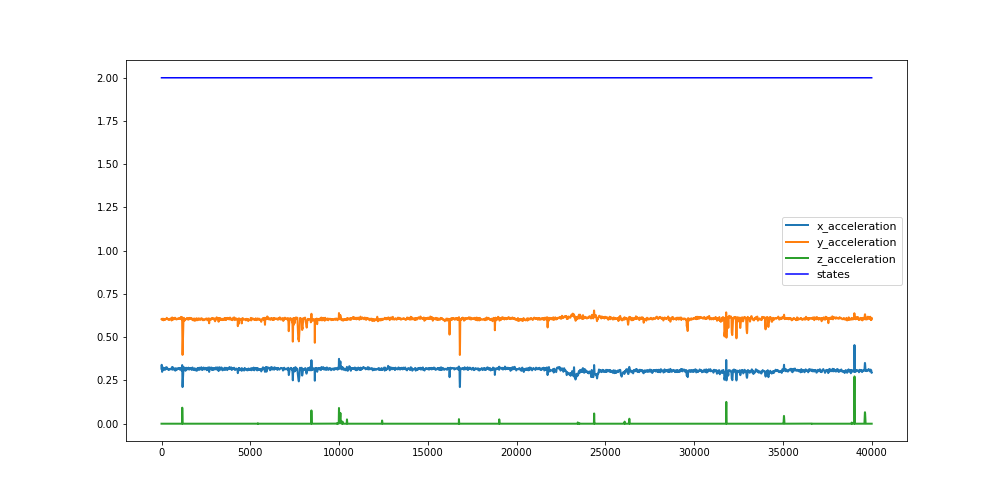
\includegraphics[width=\textwidth]{manuscript/src/figures/Ass3/Ass3_Q2_states_user_5N.png}
    \end{minipage}
    \caption{The normalized signals of x, y, and z for participant 6 and ‘Standing  Up,  Walking  and  Going  up-down  stairs’ activity. The dark blue signal indicates the different states.}
    \label{fig:Ass3_Q2_states_user_5N}
\end{figure}
\begin{figure}[H]
    \centering
    \begin{minipage}[b]{1\textwidth}
        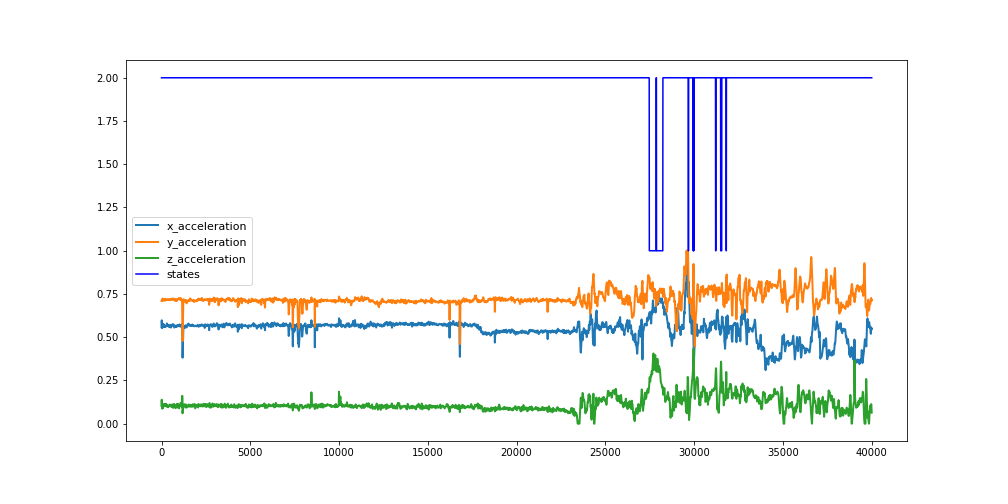
\includegraphics[width=\textwidth]{manuscript/src/figures/Ass3/Ass3_Q2_states_user_6N.png}
    \end{minipage}
    \caption{The normalized signals of x, y, and z for participant 7 and ‘Standing  Up,  Walking  and  Going  up-down  stairs’ activity. The dark blue signal indicates the different states.}
    \label{fig:Ass3_Q2_states_user_6N}
\end{figure}
\begin{figure}[H]
    \centering
    \begin{minipage}[b]{1\textwidth}
        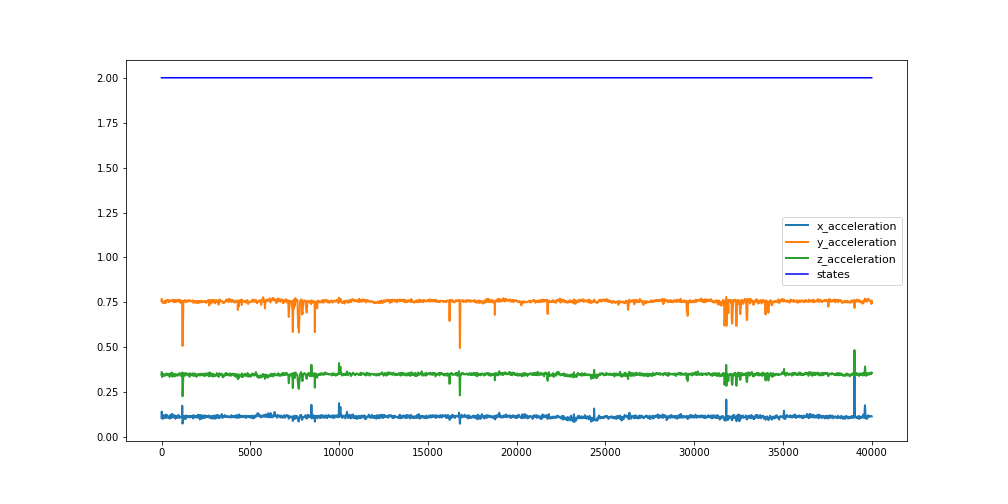
\includegraphics[width=\textwidth]{manuscript/src/figures/Ass3/Ass3_Q2_states_user_7N.png}
    \end{minipage}
    \caption{The normalized signals of x, y, and z for participant 8 and ‘Standing  Up,  Walking  and  Going  up-down  stairs’ activity. The dark blue signal indicates the different states.}
    \label{fig:Ass3_Q2_states_user_7N}
\end{figure}
\begin{figure}[H]
    \centering
    \begin{minipage}[b]{1\textwidth}
        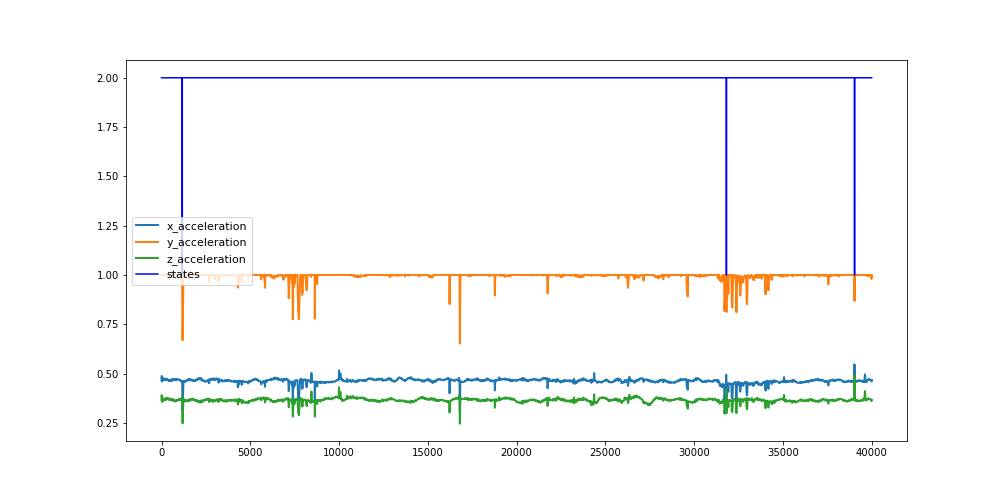
\includegraphics[width=\textwidth]{manuscript/src/figures/Ass3/Ass3_Q2_states_user_8N.png}
    \end{minipage}
    \caption{The normalized signals of x, y, and z for participant 9 and ‘Standing  Up,  Walking  and  Going  up-down  stairs’ activity. The dark blue signal indicates the different states.}
    \label{fig:Ass3_Q2_states_user_8N}
\end{figure}
\begin{figure}[H]
    \centering
    \begin{minipage}[b]{1\textwidth}
        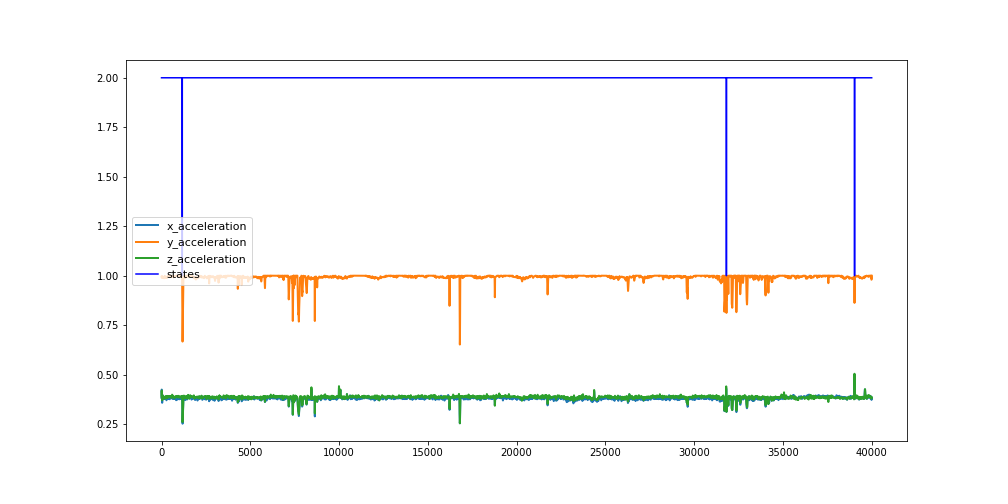
\includegraphics[width=\textwidth]{manuscript/src/figures/Ass3/Ass3_Q2_states_user_9N.png}
    \end{minipage}
    \caption{The normalized signals of x, y, and z for participant 10 and ‘Standing  Up,  Walking  and  Going  up-down  stairs’ activity. The dark blue signal indicates the different states.}
    \label{fig:Ass3_Q2_states_user_9N}
\end{figure}
\begin{figure}[H]
    \centering
    \begin{minipage}[b]{1\textwidth}
        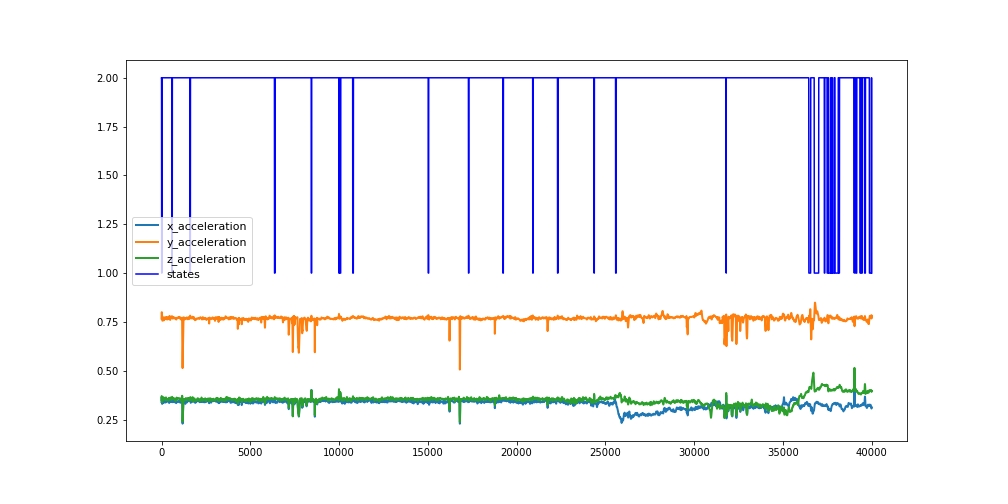
\includegraphics[width=\textwidth]{manuscript/src/figures/Ass3/Ass3_Q2_states_user_10N.png}
    \end{minipage}
    \caption{The normalized signals of x, y, and z for participant 11 and ‘Standing  Up,  Walking  and  Going  up-down  stairs’ activity. The dark blue signal indicates the different states.}
    \label{fig:Ass3_Q2_states_user_10N}
\end{figure}
\begin{figure}[H]
    \centering
    \begin{minipage}[b]{1\textwidth}
        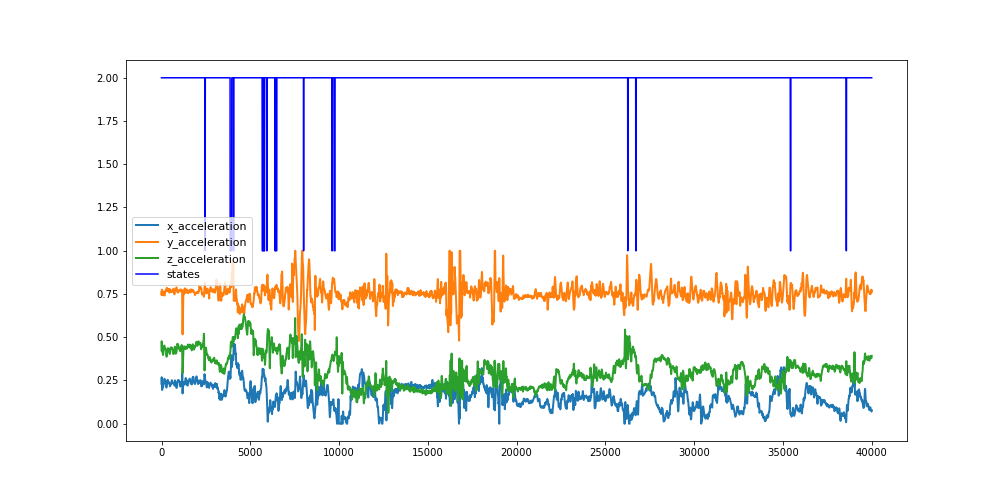
\includegraphics[width=\textwidth]{manuscript/src/figures/Ass3/Ass3_Q2_states_user_11N.png}
    \end{minipage}
    \caption{The normalized signals of x, y, and z for participant 12 and ‘Standing  Up,  Walking  and  Going  up-down  stairs’ activity. The dark blue signal indicates the different states.}
    \label{fig:Ass3_Q2_states_user_11N}
\end{figure}
\begin{figure}[H]
    \centering
    \begin{minipage}[b]{1\textwidth}
        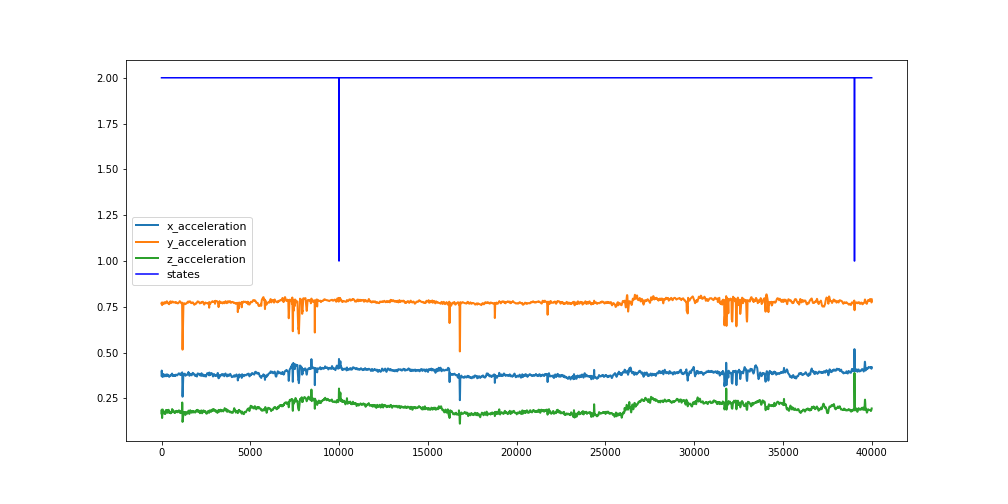
\includegraphics[width=\textwidth]{manuscript/src/figures/Ass3/Ass3_Q2_states_user_12N.png}
    \end{minipage}
    \caption{The normalized signals of x, y, and z for participant 13 and ‘Standing  Up,  Walking  and  Going  up-down  stairs’ activity. The dark blue signal indicates the different states.}
    \label{fig:Ass3_Q2_states_user_12N}
\end{figure}
\begin{figure}[H]
    \centering
    \begin{minipage}[b]{1\textwidth}
        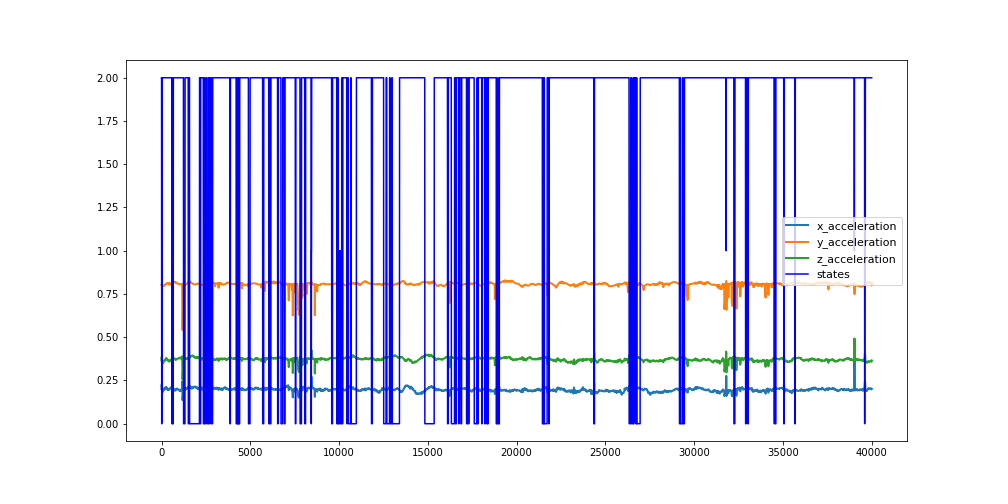
\includegraphics[width=\textwidth]{manuscript/src/figures/Ass3/Ass3_Q2_states_user_13N.png}
    \end{minipage}
    \caption{The normalized signals of x, y, and z for participant 14 and ‘Standing  Up,  Walking  and  Going  up-down  stairs’ activity. The dark blue signal indicates the different states.}
    \label{fig:Ass3_Q2_states_user_13N}
\end{figure}
\begin{figure}[H]
    \centering
    \begin{minipage}[b]{1\textwidth}
        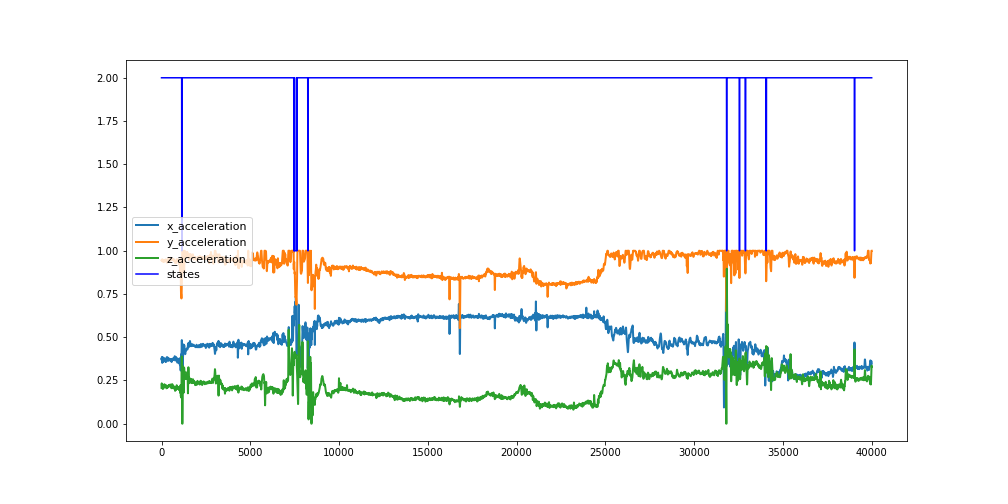
\includegraphics[width=\textwidth]{manuscript/src/figures/Ass3/Ass3_Q2_states_user_14N.png}
    \end{minipage}
    \caption{The normalized signals of x, y, and z for participant 15 and ‘Standing  Up,  Walking  and  Going  up-down  stairs’ activity. The dark blue signal indicates the different states.}
    \label{fig:Ass3_Q2_states_user_14N}
\end{figure}
%\begin{enumerate}
%\item Discrete number of hidden states (K) in the model is equal to 6, based on the labels in dataset.

%\item T shows the discrete number of observations (time points), and it is more than 100000. This number has different values according to various users.

%\item $S = (s_1, s_2, ..., s_T )$ is the hidden state sequence, which is determined by the last column of dataset (label).

%\item Observation sequence which is $O = (O_1, O_2, ..., O_T )$. In this assignment, we have three observation sequence: x, y, and z acceleration.

%\item Initial state probabilities are shown with $\Pi = (\pi_1, ..., \pi_K)$ where $\pi_i = P(s_1 = i)$ and
%$\Sigma_{i=1}^{K} \pi_i = 1$.

%\item $A = \{a_{ij} |i = 1, ..., K; j = 1, ..., K\}$is state transition probability where $a_{ij} = P(s_{t+1} = j|s_t = i)$ and $\Sigma_{j=1}^{K} a_{ij} = 1$

%\item $B = \{b_k(O_t)|k = 1, .., K;t = 1, ..., T\}$ observation probability where $b_k(O_t) = P(O_t|s_t = k)$.

%\end{enumerate}



%Typically a multivariate Gaussian distribution.

%How do we estimate the model parameters θ = {π, A, B} given one or several observation sequences

%a collection of 5 data sequences are generated. Here are two of them. They are each 500 timesteps long, and at each timestep we observe a 2-dimensional vector (black and red lines).This data was generated by 4 hidden "behaviors" (also called features). The background color specifies which behavior is active at each timepoint. Each behavior specifies a 2D Gaussian distribution, which serve as the emission parameters when the HMM is actively in that state. In this toy example, these 4 behaviors have well-separated parameters, as seen in this contour plot.